\section{Study Settings}

%\kn{This paragraph requires a motivation. The details of Boa's study must be described upfront. Something like "Boa et al.'s study performs ..... Since their study also involved a static analysis component whose impact was not measured, we perform a non-exact replication to understand the impact static analysis may have had in the results...}

\blls explored the effectiveness of test generation tools to construct sandboxes, based on sensitive APIs called by apps under analysis. Since their study also involved a static analysis component, performed by Droidfax as we described in Section~\ref{sec:introduction}, and whose impact was not measured, we replicated its work to understand the static analysis impact may have had in their results. Thus, this section present the settings of our study, whose goal is to perform this replication, and thus build a general understanding of the implications of static analysis algorithms in the results. We also investigate how static analysis can improve the performance of mining sandboxes, in the task of identifying malicious behavior.

To achieve these general goals, we intend to answer the following research questions.

\begin{enumerate}[(RQ1)]
 
 \item What is the impact of the DroidFax static analysis algorithms in the \blls?
  
 \item What is the effective performance of each test generation tool, in terms of the number of detected malware, in \blls, disregarding the DroidFax
  static analysis algorithms?

 \item What are the benefits of using tainted\kn{Is it tainted analysis or taint analysis?} analysis algorithms to complement the dynamic analysis provided by test generation tools for mining sandboxes?
\end{enumerate}

%\kn{Droidfax comes out of nowhere. We should introduce this or if already introduced earlier, remind the readers of where it stands with the Bao study in the first line of this section when describing boas study}

Answering the research questions RQ1 and RQ2 allows us to expose a possible overestimation\kn{Over estimation of what?} in performance of test generation tools for mining sandboxes,
as reported in \blls, which might introduce a possible threat to their conclusions. Answering the third research question
allows us to open up the possibility of finding new strategies for designing mining sandbox techniques, complementing the performance of
dynamic analysis through the use of static analysis algorithms.

We conducted two studies to answer the research questions above. First we replicated the \blls. However, our study differs from the original because here we isolated the effect of the DroidFax static analysis algorithms, in the task to identify malicious apps. In addition, we discarded $6$ pairs of
Android apps we were not able to instrument---out of the $102$ pairs used in the original work. We also introduced a recent test generator tool, that has not been considered at previous work, Humanoid ~\cite{DBLP:conf/kbse/LiY0C19}, and different from the original study, we expand the execution time of each test generation tool, executing each app at each tool for three minutes, and repeated all the execution more 2 times, therefore totaling three executions. The original study executed each app at each tool, for just one minute, and just one time.

The others $3$ test generation tools selected were: Droidbot~\cite{DBLP:conf/icse/LiYGC17},
DroidMate~\cite{DBLP:conf/icse/JamrozikZ16} and Monkey~\cite{Monkey}, all explored at \blls. We selected Droidbot and DroiMate because they achieved
the best performance on detecting malicious behavior at $102$ pairs of Android apps (B/M) in the \blls. At our study, we considered Droidmate-2~\footnote{In this paper, we will use Droidmate to represent Droidmate at version 2} \cite{DBLP:conf/kbse/BorgesHZ18}, because it extend the explore engine of previous version, including a new explorer set, that decide the next events to be performed. We also considered the open source tool from Google, Monkey, because it is the most widely used tool in industry \cite{DBLP:conf/sigsoft/ZengLZXDLYX16}. It is part of the Android SDK, and does not require any additional installation effort. Since Monkey was developed for stress testing, and can not perform text input, only generating
UI events, we also considered Humanoid, that emulate realistic users, creating human-like test inputs using deep learning techniques.
For the replication, we also used our benchmark tool, droidXP ~\cite{DBLP:conf/scam/CostaMCMVBC20},
which helped us to reproduce the original work.

In the second study we leverage FlowDroid~\cite{DBLP:conf/pldi/ArztRFBBKTOM14} to execute
tainted analysis algorithms in Android apps, in order to identify pairs of \emph{sources and sinks}. In this case,
our goal is to investigate the performance on detecting malicious
behavior using static taint analysis of Android apps. We use two metrics in this second study: the number
of source-sink flows that FlowDroid identifies when considering the pairs of Android apps (B/M), and the
execution time of the analysis for each app.
For both studies, we employed the same dataset $96$ pairs of Android apps (B/M),
shared by the AndroZoo \cite{DBLP:conf/msr/AllixBKT16} project. We detail our benchmark tool, droidXP, and the procedures of each study in what follows.

\subsection{The Benchmark - DroidXP}

\begin{figure*}[ht]
  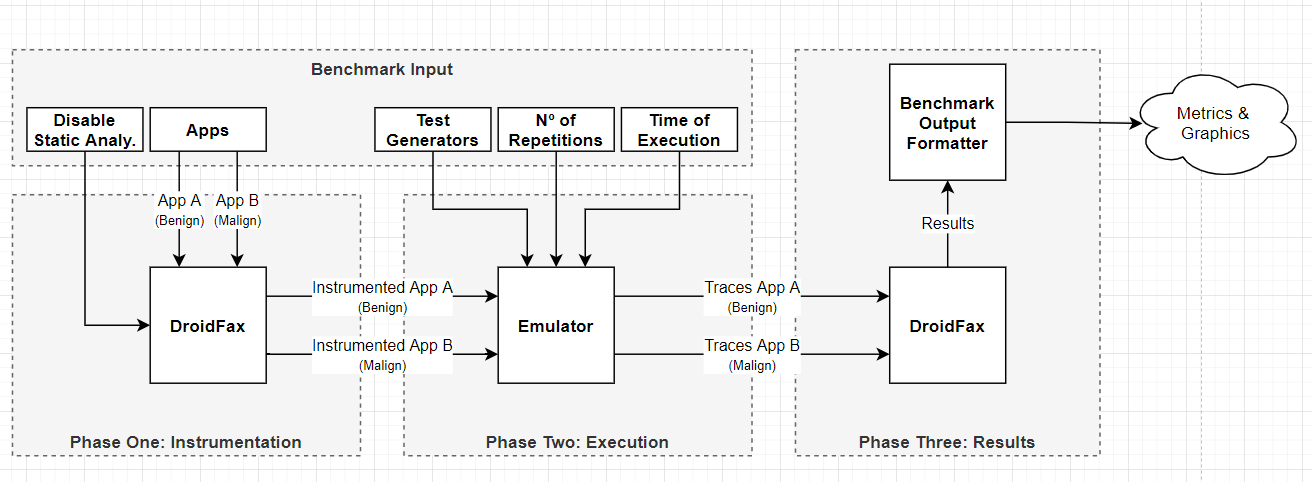
\includegraphics[width=1\textwidth]{images/benchmark4.png}
  \label{benchArq}
  \caption{Benchmark architecture}
  \label{fig:benchArq}
\end{figure*}


To systematically assess and compare test generation tools for mining android sandboxes, we used our benchmark solution, called DroidXP. It relies on a simple \emph{Command Line Interface} (CLI) that favors the execution and configuration of the benchmark. It also relies on DroidFax, that instruments Android apps and collects relevant information about their execution, like the set of sensitive APIs a given
app calls during a test execution. DroidFax also collects inter-component communication (ICC) intent  tracing  using  static  program analysis.

The DroidXP CLI provides two commands: a command that lists all test case
generation tools (executing the project with the option ``list-tools'') that had been
integrated into the benchmark; and a command that performs the execution of the benchmark,
which can be configured using the following parameters:

\begin{itemize}
    \item \texttt{-tools}: Specifies the test tools used in the experiment
    \item \texttt{-t}: Specifies the threshold (in seconds) for the execution time in the experiment
    \item \texttt{-r}: Specifies the number of repetitions used in the experiment
    \item \texttt{-output-format}: Specifies the output format
    \item \texttt{--debug}: Specifies to run in DEBUG mode (default: false)
    \item \texttt{--disable-static}: Disable DroidFax static analysis (default: false)
    
    
\end{itemize}

The DroidXP architecture relies on the pipes-and-filters architectural style \cite{architecture-book} (Figure \ref{fig:benchArq}),
and includes three main components; where each component is responsible for a specific phase of the
benchmark (instrumentation, execution, and result analysis).

\subsubsection{Phase 1: Instrumentation}

In the first phase, a researcher must define the corpus of APK files droidXP should consider during a benchmark execution. After that, DroidXP starts the DroidFax service that instruments each APK file, so that DroidXP would be able to collect data about each execution. To improve the performance of the benchmark, the instrumentation phase runs only once for each APK. In this phase, the DroidFax tool also runs some static analysis procedures.

\subsubsection{Phase 2: Execution}

In this phase, DroidXP installs an (already instrumented) APK file into
an Android emulator, and then executes a test case generation tool
during a period of time. This process repeats for every test case generation
tool and APK files. To provide repeatability of the experiment, DroidXP removes all data stored in the emulator before starting
a new execution. That is, every execution uses a \emph{fresh} emulator,
without any information that might have been kept during
previous executions. 

The benchmark is relatively easy to add new test
case generation tools. To achieve this goal, it leverage the Strategy Design pattern \cite{patterns-book}, which sets a contract between a family of classes that, in our case, abstracts the specificities for running each tool we want to integrate into DroidXP. To performance our study replication we integrated successfully all test generation tools previously mentioned into DroidXP. 

\subsubsection{Phase 3: Result Analysis}

During the execution, all the data that is required to compute the results are provided by Logcat \cite{Logcat}, one of the Android SDK's native tools and is a command-line tool that dumps a log from the Android emulator. Thus, the only part of the log that is analyzed in this phase is the messages sent by the methods inside the Android app that were instrumented on the first phase using the DroidFax tool. 

Droidfax computes the coverage each test achieved and which sensitive API was accessed during the execution of that test. That last information is required to compute the test generator performance in identifying malicious apps by spotting differences between the sensitive API accessed by each version of an app. This information is vital to the measurement of the test generator performance and qualification. After this phase, the benchmark outputs the results of the experiment, which is informing the performance of one or more testing generator tools in mining sandboxes.

\subsection{First Study: A replication \blls}

In the first study we executed the DroidXP benchmark with its
default configuration, that is, enabling the DroidFax
static analysis algorithms and the test generation tools.

We investigate the four test case generation tools described earlier and added a fake test
case generation tool (named Joker) that simulates a test tool that does not execute
the Android apps during a benchmark execution. Using this tool, the results
of the dynamic analysis are not considered and we can compute the results with
only the static analysis component of DroidFax (RQ1). Our study executed each pairs of
Android app (B/M) in each one of the five test generation tools, including Joker,
for three minutes, and for three times. We then investigate the performance of each tool to detect malicious behaviors in the sandbox modeled by the test generation tool
under analysis. Figure \ref{fig:setup} shows this experimental setup.

\begin{figure}[ht]
   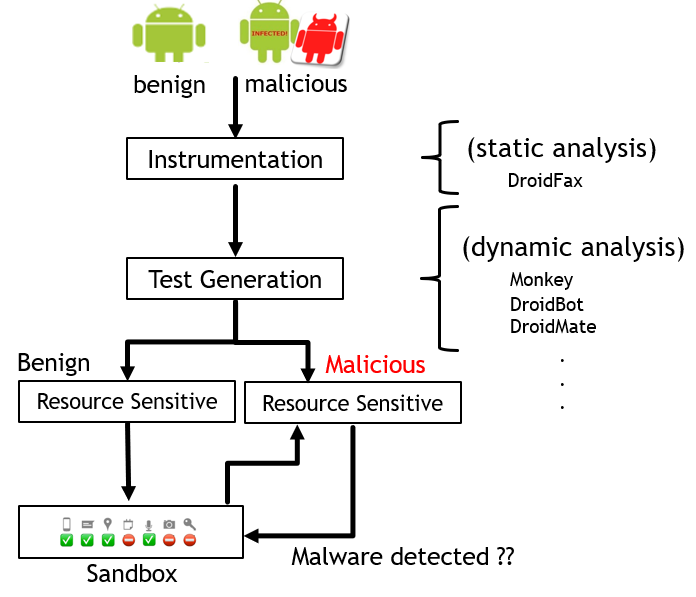
\includegraphics[width=0.45\textwidth]{images/setup2.png}
   \label{Experiment setup}
   \caption{Experiment setup}
   \label{fig:setup}
 \end{figure}

After that, we replicated the study using a configuration of DroidXP that disables the DroidFax static analysis algorithm. With this new configuration, we executed the benchmark again, using the same dataset of Android pairs apps, the same execution time, and the same test case generation tools.
The results of this replication allow us to compute the effective performance
of the dynamic analysis tools (RQ2)---that is, ignoring the influence of the
DroidFax static analysis algorithms.

\subsection{Second Study: Tainted analysis algorithms.}

To complement our initial study, we performed the tainted analysis at the same
data set from the first study. For this second study, we used
FlowDroid~\cite{10.1145/2666356.2594299}, a static flow analysis tool for Android apps.
The goal is to test accuracy of static analysis, through tainted analysis algorithms, at finding malicious behavior, and compare the results with previous study at the same data set.
In this second study, a behavior is considered malicious whenever the algorithms
detected a different set of source-sink pairs, coming from the benign and malign
versions of an Android app. 

Initially, Flowdroid mine all sources and sinks of each benign apps, and enumerates all possible data flows between them. Next, it performs the same process for the malicious version
of the correspondent app. In the final step, we compare the set of source-sink track between the benign app and its corresponding malicious app, in order to discovery some taint tracer different between the apps under analysis.

This study was useful to answer the third research question (RQ3), because it disclosed some pairs of applications with malicious behavior, that could not be detected at first study at none of the scenarios presented, evidencing that there is a benefit of new static analysis techniques, to complement the dynamic analysis provided by test generation tools, at mining sandboxes solutions. Details of studies results are at next section.





